%%%%%%%%%%%%%%%%%%%%%%%%%%%%%%%%%%%%%%%%%
% Short Sectioned Assignment LaTeX Template Version 1.0 (5/5/12)
% This template has been downloaded from: http://www.LaTeXTemplates.com
% Original author:  Frits Wenneker (http://www.howtotex.com)
% License: CC BY-NC-SA 3.0 (http://creativecommons.org/licenses/by-nc-sa/3.0/)
%%%%%%%%%%%%%%%%%%%%%%%%%%%%%%%%%%%%%%%%%

% \documentclass[paper=a4, fontsize=11pt]{scrartcl} % A4 paper and 11pt font size
\documentclass[11pt, a4paper, fleqn]{article}
\usepackage[T1]{fontenc} % Use 8-bit encoding that has 256 glyphs
\usepackage[utf8]{inputenc}
\usepackage{fourier} % Use the Adobe Utopia font for the document - comment this line to return to the LaTeX default
\usepackage{listings} % para insertar código con formato similar al editor
\usepackage[spanish, es-tabla]{babel} % Selecciona el español para palabras introducidas automáticamente, p.ej. "septiembre" en la fecha y especifica que se use la palabra Tabla en vez de Cuadro
\usepackage{url} % ,href} %para incluir URLs e hipervínculos dentro del texto (aunque hay que instalar href)
\usepackage{graphics,graphicx, float} %para incluir imágenes y colocarlas
\usepackage[gen]{eurosym} %para incluir el símbolo del euro
\usepackage{cite} %para incluir citas del archivo <nombre>.bib
\usepackage{enumerate}
\usepackage{hyperref}
\usepackage{graphicx}
\usepackage{tabularx}
\usepackage{booktabs}
\usepackage{amsmath}
\graphicspath{{./../src/imgs}}
\usepackage[table,xcdraw]{xcolor}
\hypersetup{
	colorlinks=true,	% false: boxed links; true: colored links
	linkcolor=black,	% color of internal links
	urlcolor=cyan		% color of external links
}
\renewcommand{\familydefault}{\sfdefault}
\usepackage{fancyhdr} % Custom headers and footers
\pagestyle{fancyplain} % Makes all pages in the document conform to the custom headers and footers
\fancyhead[L]{} % Empty left header
\fancyhead[C]{} % Empty center header
\fancyhead[R]{Antonio Manuel Fresneda} % My name
\fancyfoot[L]{} % Empty left footer
\fancyfoot[C]{} % Empty center footer
\fancyfoot[R]{\thepage} % Page numbering for right footer
%\renewcommand{\headrulewidth}{0pt} % Remove header underlines
\renewcommand{\footrulewidth}{0pt} % Remove footer underlines
\setlength{\headheight}{13.6pt} % Customize the height of the header


\definecolor{gray75}{gray}{0.75}
\newcommand{\hsp}{\hspace{20pt}}

\setcounter{secnumdepth}{4}




\begin{document}

	% Plantilla portada UGR
	\begin{titlepage}
\newlength{\centeroffset}
\setlength{\centeroffset}{-0.5\oddsidemargin}
\addtolength{\centeroffset}{0.5\evensidemargin}
\thispagestyle{empty}

\noindent\hspace*{\centeroffset}\begin{minipage}{\textwidth}

\centering

\includegraphics[width=0.9\textwidth]{logos/logo_ugr.jpg}\\[1.4cm]

\textsc{ \Large TRABAJO FIN DE GRADO\\[0.2cm]}
\textsc{ GRADO EN INGENIERIA INFORMATICA}\\[1cm]

{\Huge\bfseries   Titulo\\}
\noindent\rule[-1ex]{\textwidth}{3pt}\\[3.5ex]
{\large\bfseries }
\end{minipage}

\vspace{2.5cm}
\noindent\hspace*{\centeroffset}
\begin{minipage}{\textwidth}
\centering

\textbf{Autor}\\ {Antonio Manuel Fresneda Rodríguez}\\[2.5ex]
\textbf{Director}\\ {Salvador García López }\\[2cm]

\includegraphics[width=0.3\textwidth]{logos/etsiit_logo.png}\\[0.1cm]
\textsc{Escuela Técnica Superior de Ingenierías Informática y de Telecomunicación}\\
\textsc{---}\\
Granada, mes de año
\end{minipage}
\end{titlepage}


	% Plantilla prefacio UGR
	\thispagestyle{empty}

\begin{center}
{\large\bfseries Análisis de la intención de emprendimiento a través de una recogida de datos por encuestas mediante técnicas de preprocesamiento de datos y aprendizaje automático.}\\
\end{center}
\begin{center}
Antonio Manuel Fresneda Rodríguez.\\
\end{center}

%\vspace{0.7cm}

\vspace{0.5cm}
\noindent{\textbf{Palabras clave}: \textit{intención emprendedora}, \textit{aprendizaje automático}, \textit{clasificación ordinal}, \textit{clasificación multi-etiqueta}, \textit{regresión}, \textit{Python}
\vspace{0.7cm}

\noindent{\textbf{Resumen}\\
	\linebreak 
	Para que un país sea sólido económicamente, necesita empresas productivas, ya que son las que crean puestos de trabajo e impulsan el desarrollo económico.\\
	Por este motivo, detectar a aquellas personas que son capaces de crear nuevas empresa y promover que estas sean capaces de emprender y facilitar el acceso a recursos y asesoramiento necesarios puede ser un factor importante de cara al crecimiento económico de un país.\\
	La intención emprendedora se puede definir como el estado mental que provoca una atención, experiencia y acción hacia un concepto de negocio, asumiendo que esa persona no reacciona de forma automática antes los estímulos del medio, sino que procesa la información que le rodea (Bird. 1998).\\
	\linebreak
	Resolver este tipo de problemas usando técnicas clásicas puede no ser la mejor opción, ya que puede llegar a ser muy costoso en tiempo y recursos. Con el objetivo de facilitar este tipo de problemas nació el Aprendizaje Automático.\\
	El Aprendizaje Automático hace uso de unos \textbf{datos} y construye un \textbf{modelo} capaz de realizar \textbf{predicciones} tanto de los datos que ha usado como de datos nuevos.\\
	Este campo ha sufrido una gran evolución en estos últimos años, donde se han propuesto nuevos problemas, modelos y metodología, aumentando la cantidad de problemas que pueden ser resueltos.\\
	\linebreak
	Este trabajo hace uso de técnicas de Aprendizaje Automático y de unos \textbf{datos} recogidos sobre un conjunto de la población española y ecuatoriana para intentar predecir si una persona va a tener una intención emprendedora y cuales son los factores más importantes para que una persona tome este tipo de decisiones.
\cleardoublepage

\begin{center}
	{\large\bfseries Analysis of entrepreneurial intention through data collected by surveys using data preprocessing techniques and Machine Learning }\\
\end{center}
\begin{center}
	Antonio Manuel Fresneda Rodríguez\\
\end{center}
\vspace{0.5cm}
\noindent{\textbf{Keywords}: \textit{entrepreneurial intention}, \textit{machine learning}, \textit{ordinal classification}, \textit{multi-label clasification}, \textit{regression}, \textit{Python}
\vspace{0.7cm}

\noindent{\textbf{Abstract}\\
\linebreak
To keep a country solid economically, it will need profitable companies, as these are in charge of creating job posts and pushing the economic growth.\\
For these reasons, detecting people capable of creating new companies and helping them to get the resources and advice, can be important for the economic growth of a country.
Entrepreneurial intention is the mental state of mind that precedes action and directs attention toward entrepreneurial behaviors such as starting a new business. This person will use all the information around him/her and will process it to get the best decision, instead of reacting automatically to the stimuli (Bird 1998).\\
\linebreak
Solving this kind of problem using classic techniques may not be the best choice, as this can be time and resource-intensive. The goal of  Machine Learning is to ease this kind of problem. This approach will use data to build a mathematical model that will predict the data used to create the model and, most important, new data that the model hasn't used.
This field has evolved significantly during the last years, proposing new problems, models, and methodology.\\
\linebreak
This work will use Machine Learning techniques and data collected from Spanish and Ecuadorian people to find the entrepreneurial intention of a person and which are the key factors that make that choice.
\cleardoublepage
\chapter*{}
\thispagestyle{empty}

\noindent\rule[-1ex]{\textwidth}{2pt}\\[4.5ex]

Yo, \textbf{Antonio Manuel Fresneda Rodríguez}, alumno de la titulación Ingeniería Informática de la \textbf{Escuela Técnica Superior de Ingenierías Informática y de Telecomunicación de la Universidad de Granada}, con DNI 77447672W, autorizo la ubicación de la siguiente copia de mi Trabajo Fin de Grado en la biblioteca del centro para que pueda ser consultada por las personas que lo deseen.
\vspace{6cm}

\noindent Fdo: Antonio Manuel Fresneda Rodríguez
\vspace{2cm}
\begin{flushright}
	Granada a 17 de Noviembre de 2021 .
\end{flushright}

\cleardoublepage
\thispagestyle{empty}

\noindent\rule[-1ex]{\textwidth}{2pt}\\[4.5ex]

D. \textbf{Salvador García López}, Profesor del Área de Computación y Sistemas Inteligentes del Departamento de Ciencias de la Computación e Inteligencia Artificial de la Universidad de Granada.

\vspace{0.5cm}

\textbf{Informo:}

\vspace{0.5cm}

Que el presente trabajo, titulado \textit{\textbf{ Análisis de la intención de emprendimiento a través de una recogida de datos por encuestas mediante técnicas de preprocesamiento de datos y aprendizaje automático}},
ha sido realizado bajo mi supervisión por \textbf{Antonio Manuel Fresneda Rodríguez}, y autorizo la defensa de dicho trabajo ante el tribunal
que corresponda.

\vspace{0.5cm}

Y para que conste, expiden y firman el presente informe en Granada a Noviembre de 2021.

\vspace{1cm}

\textbf{El/la director(a)/es: }

\vspace{5cm}

\noindent \textbf{Salvador García López}
\pagebreak
\section*{Agradecimientos}
Me gustaría comenzar esta sección agradeciendo a mis padres el esfuerzo y la oportunidad que ellos no tuvieron para disfrutar de una educación universitaria. Muchas gracias por todo y os estoy realmente agradecido. \\
A mis hermanas, que son muy importantes para mi y que siempre han estado ahí para apoyarme y de vez en cuando para cabrearme también.
A toda mi familia, gracias abuela, abuelo, tíos, tías, primos, primas os quiero mucho y sois el pilar más importante de mi vida.\\
\linebreak
No me quiero olvidar tampoco de aquellos profesores que han formado parte en mi educación, desde la secundaria, donde creo que en ese momento no llegué a valorar lo importante que era la formación en ingles que estuve recibiendo, hasta todos aquellos docentes que me han dado clase durante todos estos años en la ETSIIT aprendiendo todo lo que me ha llevado a conseguir un trabajo en estas épocas tan complicadas y que me está haciendo muy feliz. Muchas gracias.\\
Una mención aparte para Salva, que me ha propuesto un trabajo muy interesante, me ha ayudado y animado a realizar este trabajo al que le he dedicado un montón de horas en estos meses. Muchas gracias.\\
\linebreak
Agradecer también a todos mis amigos y amigas que he estado haciendo durante todos estos años, muchas gracias por estar siempre ahí y por ser capaces de hacerme desconectar de vez en cuando. 


	% Índice de contenidos
	\newpage
	
	\tableofcontents
	
	\pagebreak

	% Introducción 
	\chapter{Introducción}
Gracias a la evolución tecnológica que hemos experimentado estos últimos años, y sobre todo a la gigantesca expansión del Internet y  a la cantidad de datos generados por dispositivos conectados a la red, ha provocado un enorme interés analizar los datos recogidos.\\
Gracias a esta información es los que nos identifican como posibles compradores de un producto, los que hacen que los coches puedan conducir por si mismos o incluso, ayuden al personal médico detectar una patología a partir de ciertos datos del paciente.
\linebreak
Se denomina \textbf{ciencia de datos} a la extracción del conocimiento de una gran cantidad datos mediante el uso del software y de  técnicas estadísticas. Este conocimiento puede ser usado para \textbf{predecir} cierta salida en función de los datos, para \textbf{detectar grupos} de datos que tengan características similares, \textbf{explicar} el comportamiento de esos datos, entre otros muchos más casos de uso. \\
\linebreak
El \textbf{Machine Learning} es un campo dentro de la ciencia de datos que se centra en la creación y entrenamiento de modelos de predicción con el objetivo de minimizar el error de salida ante una nueva entrada que el modelo no ha usado en la fase de entrenamiento.
\section{Machine Learning}
El \textbf{Machine Learning} (aprendizaje automático) es un campo de la Inteligencia Artificial que se centra en el desarrollo de técnicas que permitan a las computadores extraer conocimiento a partir de unos datos.\\
\linebreak
Estos datos pueden estar definidos de una gran número de formas, observaciones recogidas por sensores, imágenes, valoraciones de usuarios, etc. En el caso particular de este trabajo en el que se enfoca este proyecto, el \textbf{conjunto de datos} con el que se va a trabajar tiene una cantidad de \textbf{muestras} en la que cada muestra tiene un número fijo de \textbf{características} que identifican a cada muestra. Además, el conjunto de datos con el que se está trabajando, contiene una serie de \textbf{etiquetas} asignada a cada muestra.\\
\linebreak
 Usando la naturaleza de los datos, se pueden dividir los distintos tipos de técnicas que se usan en ML.
\subsection{Agrupamiento en función de los datos disponibles}
Se puede usar la naturaleza de los datos para definir varios tipos de algoritmos, ya que la metodología a seguir cuando se trabaja con datos \textbf{etiquetados} o con datos sin etiquetar es distinta. Usando esta idea, las técnicas usadas en ML pueden ser agrupadas en \textbf{aprendizaje supervisado}, \textbf{no supervisado} ó \textbf{semi-supervisado}:
\begin{itemize}
	\item \textbf{Aprendizaje supervisado:} Este conjunto de técnicas se caracteriza debido a que cada muestra tiene una ó más \textbf{etiquetas}(variable/s objetivo) y tiene como finalidad hacer uso de las características de cada muestra para \textbf{predecir} las variables objetivo de nuevas muestras que no pertenecen al conjunto de datos inicial. Alguna de las tareas que entran dentro de este grupo son \textbf{Clasificación} ó \textbf{Regresión}
	\item \textbf{Aprendizaje no supervisado:} A diferencia del anterior, las técnicas de aprendizaje no supervisado se diferencian en que las muestras \textbf{no están etiquetadas}, por lo que no se puede \textbf{predecir} ninguna variable. Estas técnicas se caracterizan por ser capaces de \textbf{reconocer patrones} dentro del conjunto de datos, etiquetando las nuevas entradas haciendo uso de ellos. La tarea más común es \textbf{Clustering}
\end{itemize}
Anteriormente se han mencionado tareas como \textbf{clasificación}, \textbf{regresión} o \textbf{clustering}, en la siguiente sección se va a profundizar más, explicando en que consiste cada una y que objetivos tienen.
\subsection{Agrupamiento en función de la tarea}
\begin{itemize}
		 \item \textbf{Clasificación:} Como se mencionó previamente, esta tarea tiene sentido cuando se usa un conjunto de datos que está etiquetado. El objetivo principal de clasificación consiste en dada una nueva muestra, \textbf{predecir} una o varias etiquetas en función del conjunto de datos que se ha usado. Estas etiquetas suelen ser variables \textbf{discretas}
		 \item \textbf{Regresión:} A diferencia de clasificación, donde las variables objetivo son discretas, en este caso las variables objetivo son continuas. El propósito de estas técnicas es el de predecir un \textbf{valor} para nuevas muestras.
		 \item \textbf{Clustering:} El objetivo es el de detección de patrones usando datos no etiquetados.
\end{itemize}
Dentro de las tareas de clasificación, se pueden dividir en varios grupos. En la siguiente sección se va a explicar los distintos tipos de clasificación, ya que ayudara a entender la naturaleza del problema que se esta tratando en este trabajo.
\section{Tipos de clasificación}
Como ya se ha mencionado previamente, clasificación usa un conjunto de datos para predecir un valor de una o mas variables de salida. Según el tipo de variable que se va a predecir, se pueden identificar los siguientes tipos de clasificación:
\subsection*{Clasificación binaria}
Este es el tipo de clasificación más sencilla, ya que la variable objetivo solo va a tener dos posibles valores. Estos valores se conocen como clase positiva (1) ó clase negativa (0). De aquí viene el nombre de clasificación \textbf{binaria}, ya que la variable objetivo es binaria.\\
Ejemplos de este tipo de clasificación son detectar si un mensaje es spam, si en función de ciertos valores una bomba de agua puede fallar, o detectar si un cliente de un banco va a tener deudas usando ciertos parámetros.
\begin{figure}[H]
	\centering
	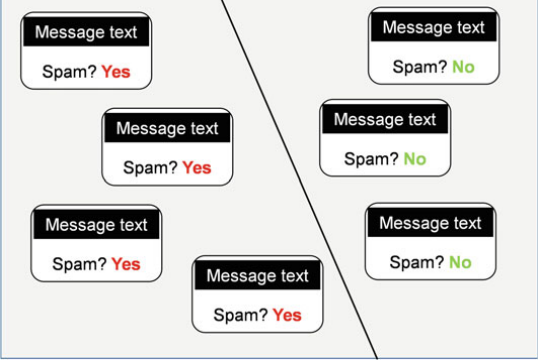
\includegraphics[scale=0.4]{binary-class.png}
	\caption{Ejemplo de clasificación binaria: Identificar si un correo electrónico es spam.}
	\label{fig:bclass}
\end{figure}
\subsection*{Clasificación multi-clase}
Los conjuntos de datos que se usan en clasificación multi-clase son una generalización del caso de clasificación binaria, ya que al igual que la clasificación binaria, solo existe una única variable objetivo, siendo la principal diferencia que la variable objetivo puede tener cualquier valor dentro de un conjunto de posibles valores. Es importante destacar que estos valores son \textbf{discretos} y \textbf{finitos}. El ejemplo más conocido de este tipo de clasificación es la \textbf{clasificación de la flor del Iris}, donde en función de la longitud y anchura del sépalo y del pétalo, se predice si la flor es setosa, virgínica o versicolor.
\begin{figure}[H]
	\centering
	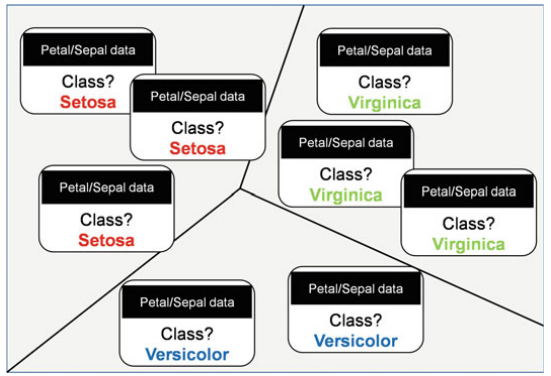
\includegraphics[scale=0.4]{multiclass-class.png}
	\caption{Ejemplo de clasificación multi-clase: Clasificación de la flor del Iris}
	\label{fig:mcclass}
\end{figure}
\subsection*{Clasificación ordinal}
Clasificación ordinal es un caso particular de clasificación multi-clase donde existe una relación de orden entre las clases.\\
Un ejemplo de este tipo de clasificación es el de predecir la valoración de una película, predecir las preferencias de una persona (en desacuerdo, de acuerdo).
\subsection*{Clasificación multi-etiqueta}
A diferencia de los anteriores tipos de clasificación, cada muestra tiene un \textbf{conjunto de variables objetivo} en lugar de una única variable. En este caso, el número de variables objetivo es fijo, siendo estas de tipo binario. A cada combinación distinta de valores se conoce como \textit{labelset}.\\
Los algoritmos que usados para este tipo de problema deben de ser capaces de realizar varias predicciones, ya sea modificando los datos originales o adaptando algoritmos de clasificación binaria o multi-clase.\\
\linebreak
Un ejemplo de este tipo de clasificación puede ser el de comprobar si una imagen contiene ciertos elementos. 
\begin{figure}[H]
	\centering
	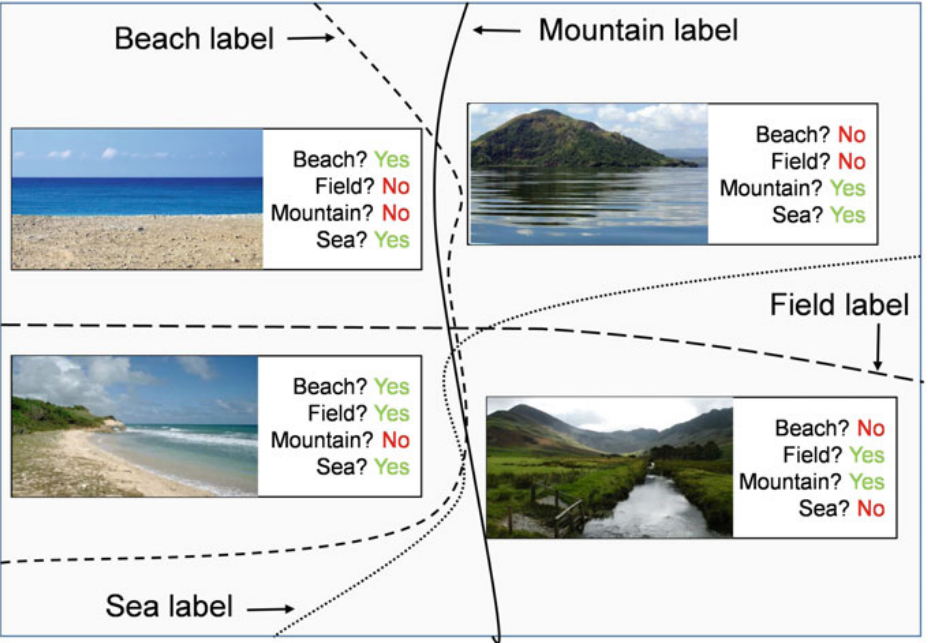
\includegraphics[scale=0.4]{multilabel-class.png}
	\caption{Ejemplo de clasificación multi-etiqueta: Clasificar si una imagen contiene ciertos elementos.}
	\label{fig:mlclasss}
\end{figure}
\subsection*{Clasificación multi-dimensional}
Al igual que la clasificación multi-clase es una generalización del caso binario, la clasificación multi-dimensional es una generalización de la clasificación multi-etiqueta.\\
En este caso, cada muestra tiene un conjunto fijo de variables objetivo que pueden tomar cualquier valor dentro de un conjunto de posibles valores. 
\section{Introducción al problema}
Pongámonos en situación de una persona dentro del departamento de marketing de una empresa que se centra en la creación de cursos. Determinar que variables son capaces de definir la intención emprendedora de una sección de la población podría ser beneficioso para la empresa, ya que podrían crear esos cursos enfocándose en aquellas variables más importantes (edad, estudios, ......) para que de una forma más eficiente captar a interesados, cambiar ciertas características de esos cursos para que sean accesibles a gente con más interés y, en definitiva, optimizar los recursos empleados en esos cursos para incrementar el beneficio.\\

	\pagebreak
	% Descripción del problema y hasta donde se llega

\pagebreak
	\section{Pre-procesamiento}
\subsection{Introducción}
Cualquier problema en ciencia de datos, comienza con un estudio exhaustivo de los datos proporcionados y realizar un \textbf{procesamiento} previo.
Si este paso es omitido, los algoritmos no se comportarán de forma óptima, debido a  que van a lidiar con unos datos que tendrán valores perdidos, que no estén normalizados, datos des-balanceados, irrelevantes, entre otras problemas. El objetivo de esta fase, es realizar ciertas transformaciones sobres los datos en bruto filtrando esta información para que los algoritmos no tengan que enfrentarse a estos problemas.
\subsection{Análisis exploratorio de los datos}
Para comenzar, se empezó leyendo la documentación aportada con los datos, la cual contenía los siguientes campos:
\begin{itemize}
	\item \textbf{Nombre:} Nombre de la característica.
	\item \textbf{Descripción:} Breve resumen explicando el origen de la característica o el enunciado de la pregunta en la encuesta.
	\item \textbf{Valores:} Tipo y/o rango que toma la característica.
\end{itemize}

Esta información es muy útil, ya que aparte de darnos un poco más de conocimiento del objetivo que queremos alcanzar con estos datos, nos da información de algunas características redundantes.

\begin{table}[H]
	\begin{tabular}{|l|l|l|}
		\cline{1-3}
		CF9  &	Normalmente es posible reducir...&	Respuesta: Verdadera/Falsa. \\ \cline{1-3}
		QF9	& Variable creada a partir de CF9.  & Valor 1 si la respuesta es correcta, 0 si no. \\ \cline{1-3}
	\end{tabular}
	\label{tab:columnas_iguales}
	\caption{Comparación de dos características redundantes.}
\end{table}
Como podemos ver, estas dos columnas contienen información redundante, ya que siendo una respuesta de tipo verdadero o falso, tenemos dos columnas con la misma información. Este caso se repite en varios casos, y en todos ellos se ha optado por dejar unicamente la que tiene los valores numéricos.\\
\linebreak
El siguiente paso ha sido el de obtener las columnas que se van a usar como predictores.
La peculiaridad de este conjunto de datos tenemos 7 columnas que van a ser las que los algoritmos tienen que intentar predecir. De estas 7 columnas tenemos 6 de ellas que son de tipo ordinal, almacenando la opinión (en escala Likert) que ha tenido el entrevistado sobre la pregunta en concreto. La ultima de estas columnas es la media de las 6 columnas.\\
 A continuación se muestra una tabla con la ocurrencia de cada valor para las columnas que vamos a usar:\\
\linebreak
 \begin{figure}[H]
 	 \centering
	 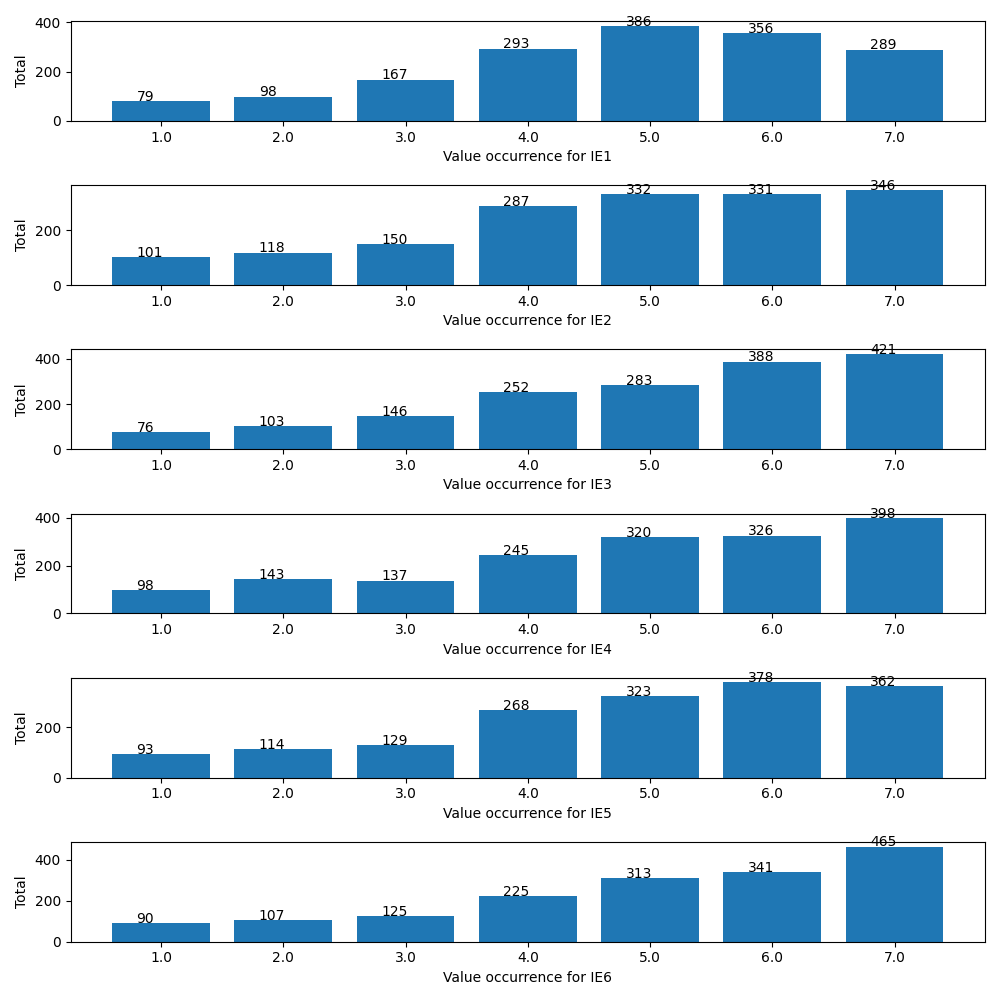
\includegraphics[scale=0.5]{src/value_occurrences.png}
	\caption{Conteo de valores para las columnas usadas como predictores}
	\label{tab:ocurrencia_valores}
\end{figure}
Una vez leída esta documentación y detectados algunos casos de columnas con información redundante, se cargaron los datos y se sacaron una serie de métricas. Estamos ante un conjunto de datos formados por un total de 1672 ejemplos y con 246 características (antes de realizar cualquier tipo de procesamiento), las cuales pueden ser de tipo entero, flotante o categóricas.
\pagebreak
\subsection{Pre-procesado de datos}
En este paso también se han borrado aquellas columnas las cuales corresponden a respuestas de tipo abierta. Estas características pueden llegar a contener un valor único por cada uno de los ejemplos que tenemos. En un principio, van a ser descartadas, pero en fases siguientes se podría realizar un procesamiento más exhaustivo sobre dicha columna, agrupando ciertos valores y reduciendo así la complejidad. Cabe destacar que esta información no se esta perdiendo totalmente, ya que tenemos en todos los casos una nueva columna la cual contiene si la persona respondió correctamente o no a dicha pregunta. \\
\linebreak
Un caso particular que se detectó en esta fase, fue el de las características \textbf{BFx} y \textbf{BFxAdaptada} (hay un total de 4 columnas de este tipo). Las primeras columnas de este tipo, solo contenían la respuesta las personas que realizaron la entrevista en un único año, mientras que las columnas del segundo tipo contenían la respuestas de los dos años. Antes de eliminar las columnas del primer tipo, se realizo una comprobación para ver si realmente los datos comunes entre las dos columnas eran los mismos para así asegurar que no se están perdiendo datos.
\linebreak
El siguiente paso, ha sido analizar los valores únicos de cada variable, esto nos permitió detectar valores no validos. Se encontró los siguientes casos de valores nó validos:
\begin{itemize}
	\item \textbf{Valores perdidos especificados como espacios:} Si no procesamos estos valores, el algoritmo puede detectarlo como un valor válido, introduciendo así ruido en el modelo. Estos valores se cambiaron por \textit{NaN}.
	\item \textbf{Valores perdidos especificados como "\textit{No contesta}":} Estos valores se ven sobre todo en columnas con datos ordinales. El enfoque que se ha escogido ha sido el de cambiarlas por \textit{NaN}.
	\item \textbf{Valores inválidos en la columna "\textit{género}":} Según la documentación, los únicos valores que forman esta columna son \textit{hombre} y \textit{mujer}, pero dentro del conjunto de datos se detectan valores como \textit{si} y \textit{no}. No podemos saber si la persona que contestó la encuesta se equivocó ó le llegó una versión distinta de la encuesta, así que, estos valores dentro de la columna \textit{género} se reemplazaron por \textit{NaN}.
	\item \textbf{Valores binarios codificados como strings:} Este caso no es necesariamente un valor no válido, pero se decidió cambiar estos valores binarios codificados como \textit{sí} o \textit{no} por \textit{1} y \textit{0} respectivamente. Con este cambio no vamos a perder información y vamos a ahorrarnos el codificar ciertas columnas en fases posteriores.
\end{itemize}

El siguiente paso ha sido el de obtener las columnas con una alta correlación. Hemos considerado como alta correlación, aquellas columnas cuya correlación sea mayor que 0.9\\
El resultado ha sido: \\
\begin{table}[H]
	\centering
	\begin{tabular}{|l|l|l|l|}
		\cline{1-3}
		Columna 1             & Columna 2              & Correlación  \\ \cline{1-3}
		IF1.6jTiene    	      &  FI\_Insur             &  1.000000    \\ \cline{1-3}
		FinLit total(1-19)    & FinLit normaliz        & 1.000000     \\ \cline{1-3}
		ConFin(1\_7)          & ConFin(1\_8)           &  0.987110    \\ \cline{1-3}
		FinBehSinBorrow (1-6) & FinBeh con borrow(1-7) &  0.948779    \\ \cline{1-3}
	\end{tabular}
	\label{tab:correlacion}
	\caption{Matriz de correlación}
\end{table}
Volviendo a revisar la documentación, tenemos las siguientes descripciones:
\linebreak
\begin{itemize}
	\item \textit{FI\_Insur}: Si tiene Productos de seguro: contrato de seguros (IF1.6jTiene). Valor 1 cuando tiene alguno, en caso contrario toma valor 0.
	 \item \textit{FinLit normaliz}: Puntuación de Competencia financiera normalizada calculado dividiendo entre 19 y multiplicando por 100. Indica el porcentaje de competencia financiera general sobre 100. (columna \textit{FinLit total}).
	 \item \textit{ConFin(1\_7)}: Variable global de Conocimientos financieros generales sumando QF3 a QF9. \textit{ConFin(1\_8)} suma de QF2 a QF9.
	 \item \textit{FinBehSinBorrow (1-6)}: Suma de las variables de comportamiento financiero excepto Borrow. \textit{FinBeh con borrow(1-7) } introduce Borrow.
\end{itemize}
Como vemos, viendo la explicación de las variables, podemos prescindir de ciertas columnas. En este caso se han descartados las características de la columna 2.\\
\linebreak
Por último, se ha dividido el conjunto de datos en los conjuntos de entrenamiento y test.
\linebreak
A continuación, se va a explicar qué algoritmos se han usado para imputación de valores perdidos, codificación de características categóricas y normalización, etc. En cada subsección de \textbf{\ref{sec:algoritmos}-\nameref{sec:algoritmos}}, se especifica que algoritmos han sido aplicados a cada modelo.

\subsubsection{Valores perdidos}
Un valor perdido es aquel para el que en una variable determinada, no consta en una o más muestras de conjunto de datos. En caso de que se trabaje con un conjunto de datos con valores perdidos, se puede optar por:
\begin{itemize}
	\item \textbf{Eliminar} aquellas muestras que contengan valores perdidos.
	\item \textbf{Imputar} los valores perdidos en función de del resto de muestras.
\end{itemize}

La opción de eliminar las muestras tiene la ventaja de que no se está introduciendo información artificial al conjunto de datos, manteniendo así las características originales, pero claramente tiene una desventaja, y es que se está eliminando información, pudiendo impactar en el comportamiento de los algoritmos.\\
\linebreak
La segunda opción implica el estar modificando el conjunto de datos con muestras \textbf{artificiales}, alterando así las características del conjunto de datos pero sin eliminar información.\\
Estas muestras artificiales se pueden usar estadísticos como la \textbf{media}, \textbf{moda} de la variable con valores perdidos. El uso de estos estadísticos en esta fase tiene una gran desventaja: Solo se está usando la información de la propia variable, cabiendo la posibilidad que una o más variables del resto del conjunto de datos influyan en la variable que se está tratando. \\
\linebreak
Para evitar la desventaja del uso de estadísticos, puede usarse un algoritmo de machine learning para \textbf{predecir} que valor tendría el valor perdido de la variable que se está analizando. \\
\linebreak
Para imputar valores perdidos en una primera iteración del proceso, se ha usado el algoritmo KNN. Este algoritmo está explicado con más profundidad en la sección \textbf{\ref{alg:knn}-\nameref{alg:knn}} de este mismo documento, resumiendo, dada una muestra nueva,  este algoritmo calcula la \textbf{diferencia} entre la nueva muestra y \textbf{todas} las muestras del conjunto de datos, seleccionando la variable de salida de las $K$ muestras más cercanas y asignando el valor predicho en función de las variables de salida seleccionadas.
\subsubsection{Codificación de variables categóricas}
Existen algoritmos que no aceptan variables categóricas (Redes Neuronales, KNN, SVM, etc) por lo que un paso muy importante antes de usar estos algoritmos, es de adaptar el conjunto de datos para que el algoritmo funcione. \\
Una opción puede ser eliminar aquellas variables categóricas, pero se podría estar perdiendo información importante. Para usar estos algoritmos sin eliminar información lo más normal es \textbf{codificar} las variables categóricas.\\
Existen dos opciones para la codificación:
\begin{enumerate}
	\item \textbf{Codificación por etiqueta:} Cada valor único de la variable se sustituye por un valor entero.
	\item\textbf{Codificación \textit{one-hot }:} Se cambia la variable categórica por una serie de variables \textit{dummies}
\end{enumerate}

La codificación por etiqueta tiene la ventaja que es la más natural para los humanos y podría parecer suficiente, pero tiene una gran desventaja: Los valores enteros tienen una \textbf{relación de orden} entre cada valor. Los algoritmos de machine learning son capaces de entender esta relación de orden y perjudicar la eficacia del modelo.\\
\linebreak
La codificación \textit{one-hot}  crea una variable por cada valor único de la variable a codificar. Cada nueva variable se asocia con un valor único y tendrá el valor $1$ cuando el valor para esa muestra sea el asociado, fijando el valor a $0$ para el resto de nuevas variables. Un ejemplo sería el siguiente:\\
Dada el siguiente conjunto de datos de ejemplo:\\
\begin{table}[H]
	\centering
	\begin{tabular}{|c|c|}
		\cline{1-2}
		ID    &	  Vehículo.  \\ \cline{1-2}
		0	  &   Moto       \\ \cline{1-2}
		1	  &   Camión     \\ \cline{1-2}
		2     &   Coche      \\ \cline{1-2}
		3	  &   Moto       \\ \cline{1-2}
	\end{tabular}
	\caption{Conjunto de datos de ejemplo.}
	\label{tab:conjunto_ejemplo}
\end{table}
Si usamos codificamos la variable \textit{vehículo} usando la etiqueta, estaríamos imponiendo una relación de orden sobre \textit{moto, camión y coche}, pudiendo "confundir" al algoritmo. Si usamos la codificación \textit{one hot}, el conjunto quedaría:

\begin{table}[H]
	\centering
	\begin{tabular}{|c|c|c|c|}
		\cline{1-4}
		ID  & Vehículo\_moto & Vehículo\_camión & Vehículo\_coche. \\ \cline{1-4}
		0	& 1  			 & 0				& 0		           \\ \cline{1-4}
		1	& 0				 & 1				& 0 			   \\ \cline{1-4}
		2   & 0 			 & 0 				& 1				   \\ \cline{1-4}
		3   & 1 			 & 0 				& 0			       \\ \cline{1-4}
	\end{tabular}
	\caption{Conjunto de datos de ejemplo tras codificar}
	\label{tab:conjunto_ejemplo_cod}
\end{table}
Como se ve en la tabla \ref{tab:conjunto_ejemplo_cod}, se ha transformado la columna \textit{vehículo} en tres columnas distintas, tomando el valor 1 cuando el valor de la variable sin codificar coincide con la variable asignada para ese valor. \\
\linebreak
Este modelo tiene una desventaja clara, y es se van a crear tantas columnas como valores único tenga la variable a codificar, esto puede incrementar significativamente el tamaño del conjunto de datos, pudiendo impactar en el rendimiento de los modelos.

	\pagebreak
\pagebreak

\pagebreak
\section{Algoritmos}
\label{sec:algoritmos}
\subsection{Introducción}
En esta sección vamos a explicar que algoritmos se han usado después del pre-procesamiento inicial.\\
Existe un teorema llamado\textbf{ \textit{No-Free-Lunch}} que afirma no existe un algoritmo que resuelva los problemas de machine learning mejor que otro.\\
Partiendo de esta idea, el objetivo principal de esta sección es el de comprobar el comportamiento de una serie de modelos elegidos. \\
De estos modelos, algunos se adaptaran mejor que otros para los datos con los que se trabajan. Una vez analizado el comportamiento, podremos decidir que algoritmos vamos a usar y que algoritmos van a ser descartados. \\
\linebreak
Para el caso especifico con el que se está trabajando, vemos que es un problema bastante peculiar, ya que esta formado por varias variables objetivo de tipo ordinal, añadiendo una nueva característica siendo esta la\textbf{media} de estas variables.\\
Para esta sección, se ha usado la media y se ha planteado un problema de \textbf{regresión}, en el que algoritmo, dada una entrada predecirá que valor medio de emprendimiento tiene esa persona.

\subsection{Métricas}
Para comprobar el comportamiento de nuestro modelo se usan \textbf{métricas}.  Las métricas que se han usado son \textit{\textbf{Coeficiente de determinación}} (se denota como $R^2$), \textit{\textbf{Desviación de Poisson}} y \textit{\textbf{Error cuadrático medio}}
\subsubsection{Coeficiente de determinación}
Se define como \textbf{coeficiente de determinación} como la proporción de la varianza total explicada por la variables independientes del modelo. Proporciona una indicación de como de bueno es un ajuste y por tanto, una medida de como de bueno es el modelo cuando predice nuevas muestras.\\
\linebreak
Matemáticamente, se define el coeficiente de determinación como:
\[
	R^2 (y, \hat{y}) = 1 - \frac{\sum_{i=1}^{n}(y_i - \hat{y}_i)^2}    {\sum_{i=1}^{n} (y_i - \overline{y})^2}
\]

Donde:
\begin{itemize}
	\item $y$ es el conjunto de valores reales para las variables objetivo.
	\item $\hat{y}$ es el valor predicho para los valores objetivo.
	\item $\hat{y}_i$ es la predicción de la  i-ésima muestra.
	\item $y_i$ es el valor real de la i-ésima muestra.
	\item $\overline{y} = \frac{1}{n} \sum_{i=1}^{n} y_i$.
	\item $n$ es el numero de muestras del conjunto.
\end{itemize}
insertar graficos explicando varianza,  etc
\subsubsection{Desviación de Poisson}
\subsubsection{Error cuadrático medio}
El error cuadrático medio de un estimador mide el promedio de los errores al cuadrado.  \\
Matemáticamente, se define el error cuadrático medio como:
\[
	MSE(y,\hat{y}) = \frac{1}{n} \sum_{i=1}^{n} (y_i - \hat{y}_i) ^2
\]
Donde:
\begin{itemize}
	\item $y$ es el conjunto de valores reales para las variables objetivo.
	\item $\hat{y}$ es el valor predicho para los valores objetivo.
	\item $\hat{y}_i$ es la predicción de la  i-ésima muestra.
	\item $y_i$ es el valor real de la i-ésima muestra.
	\item $n$ es el numero de muestras del conjunto.
\end{itemize}
\subsubsection{Conjuntos de validación}
Para ver el comportamiento de un modelo, se puede definir un conjunto de entrenamiento para entrenar el modelo que se ha seleccionado y un conjunto de test para comprobar el comportamiento con datos que el algoritmo no conoce.  Aunque a primera vista esta parece una técnica correcta, tiene varios inconvenientes:
\begin{itemize}
	\item Cuando se ajustan los hiper-parámetros de los modelos,  se podría llegar a ajustar el modelo al conjunto de test, produciendo un sobre-ajuste.
	\item Solo se esta usando una parte de los datos para validar el modelo, nada asegura que el conjunto de test sea representativo del conjunto de datos con el que se está trabajando.
\end{itemize}
Para solventar estas y algunos otros problemas que que tiene esta metodología, se usa la \textbf{validación cruzada}.\\
\linebreak
En vez de usar el conjunto de entrenamiento para entrenar un único modelo, se divide el conjunto de entrenamiento en $k$ partes, entrenando $k$ modelos usando $k-1$ subconjunto y usando el restante como de test. \\
 \begin{figure}[!htbp]
	\centering
	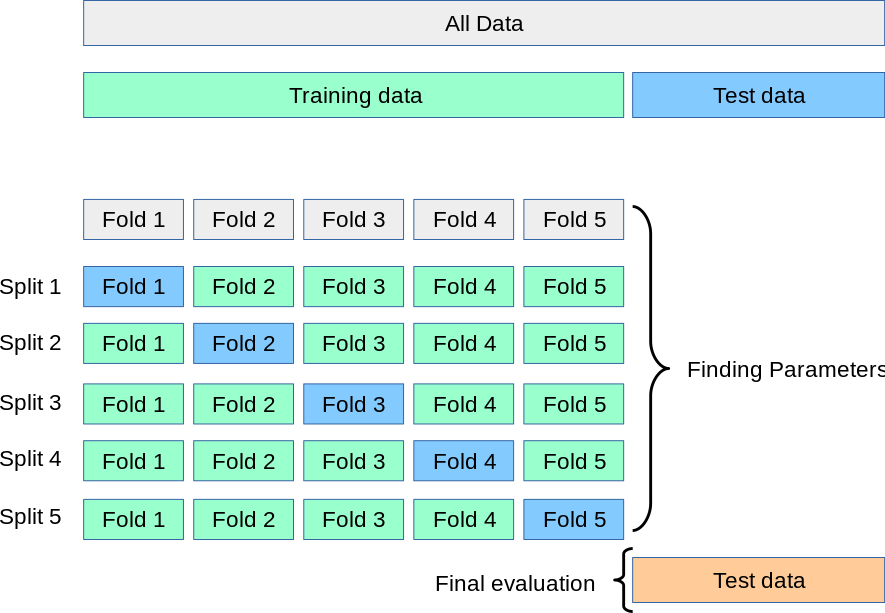
\includegraphics[scale=0.4]{grid_search_cross_validation.png}
	\caption{Ejemplo de validación cruzada con $k=5$}
	\label{fig:cross-validation}
\end{figure}
\linebreak
Como se aprecia en la figura \ref{fig:cross-validation},  se ha dividido el conjunto de datos en 5 conjuntos (folds), usando en cada iteración 4 para entrenar el modelo y uno para verificar con datos que el modelo no ha visto. Finalmente, se usa el conjunto de test (habiendo entrenado previamente el modelo con todo el conjunto de entrenamiento).
\subsubsection{Gráficos}
Además del uso de las métricas mencionadas previamente, se han creado las siguientes gráficas para visualizar los errores que esta haciendo un modelo en concreto. Esto ayuda a la toma de decisiones en fases siguientes.\\
Las gráficas que se han desarrollado son las siguientes:
\begin{itemize}
	\item Gráfico de dispersión de errores.
	\item Cantidad de errores por rango. (probablemente sea mejor cambiar este nombre, pero es el nombre que se me ocurrió)
\end{itemize}
El gráfico de dispersión de errores consiste en mostrar en la misma gráfica el valor real de las variables objetivo y el valor predicho por nuestro modelo. Esto nos permite ver como de juntos están las predicciones, identificando así en que zonas el algoritmo se está equivocando más frecuentemente.\\
 \begin{figure}[!htbp]
	\centering
	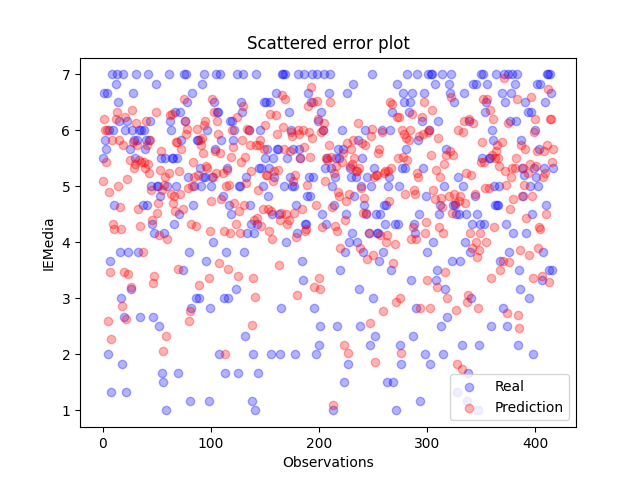
\includegraphics[scale=0.6]{scattered.png}
	\caption{Ejemplo de gráfico de dispersión de errores}
	\label{fig:scattered_example}
\end{figure}
\linebreak
El segundo gráfico consiste en lo siguiente:
Los modelos que han sido entrenados están prediciendo valores medios. El proceso seguido para realizar estos gráficos ha sido el de obtener la diferencia entre los valores reales y los valores predichos. Si esa diferencia es mayor que un umbral (generalmente se ha usado 0.5), esa predicción se ha considerado como error. En ese caso, se ha considerado el valor real redondeado y se han contado el número de errores para cada valor redondeado.\\
Usando esta gráfica, se puede identificar fácilmente en que rangos los modelos están fallando.\\
\linebreak
 \begin{figure}[!htbp]
	\centering
	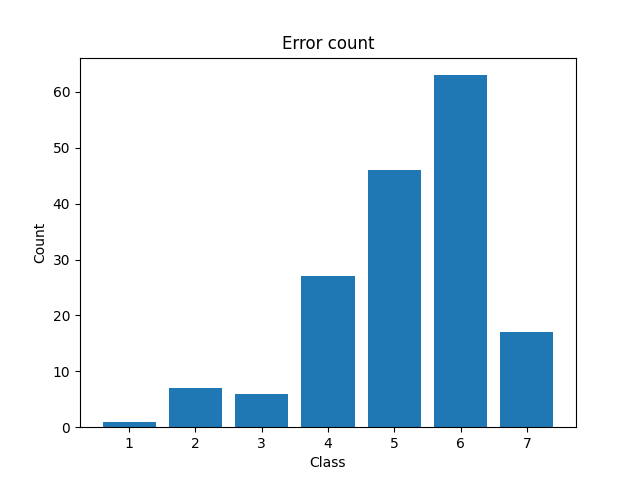
\includegraphics[scale=0.6]{error_hist.png}
	\caption{Ejemplo de gráfico de errores por rango}
	\label{fig:error_hist_example}
\end{figure}
\\
\pagebreak
\subsection{Árboles de decisión}
\label{alg:dec_tree}
Los árboles de decisión son modelos que predicen la variable objetivo usando reglas del tipo \textit{si variable cumple condición entonces } inferidas a partir de los datos con los que se entrena el algoritmo.\\
Los árboles de decisión ofrecen ciertas ventajas:
\begin{enumerate}
	\item Son modelos fáciles de interpretar y pueden ser visualizados.
	\item Son capaces de trabajar con variables categóricas y numéricas.
	\item introducir alguna ventaja más
\end{enumerate}
Sin embargo, estos modelos también presentan ciertas desventajas:
\begin{enumerate}
	\item Algoritmos que tienden al sobre-aprendizaje.
	\item No soportan valores perdidos.
	\item No trabajan bien con conjuntos de datos des-balanceados.
\end{enumerate}
Se ha seleccionado este algoritmo ya que es un algoritmo que a parte de predecir nuevos valores, puede proporcionar información extra sobre conjunto de datos (importancia de variables, variables que definen cierto grupo, etc).
\subsubsection{Procesado de datos}
Antes de ejecutar la fase de entrenamiento, hay que modificar los datos para adaptarlos a las limitaciones que algoritmo impone. En este caso,  los árboles de decisión no admiten valores perdidos y debido a ciertas limitaciones de la librería que se está usando, los árboles de decisión no son capaces de trabajar con variables categóricas.\\
Las modificaciones que se han hecho previamente son: (por orden)
\begin{enumerate}
	\item \textbf{Imputación de valores perdidos}
	\item \textbf{Transformación de variables categóricas a numéricas}
\end{enumerate}
 Por este motivo, se ha tenido que introducir una fase extra transformando las variables categóricas en numéricas.
\subsubsection{Resultados}
Antes de mostrar los resultados, hay que destacar que cuando se entrena un árbol de decisión sin limitar los parámetros, este va a seguir separando los datos de entrenamiento hasta que no pueda realizar más divisiones. Para encontrar el árbol óptimo, primero se ha entrenado el árbol por defecto y se han obtenido los parámetros. Esos parámetros se han establecido como limite, se han entrenado varios árboles con distintos parámetros (sin superar el límite establecido por el primer modelo) y se ha escogido el que mejores resultados obtenía. Los parámetros que mejor resultados dieron son: \\
\begin{itemize}
	\item \textbf{Profundidad máxima:} Limita la profundidad (cantidad de preguntas) del árbol. El mejor valor ha sido \textbf{8}
	\item \textbf{Máximo número de hojas:} Máximo numero de hojas (grupos en el último nivel de una rama). El mejor valor ha sido \textbf{16}
\end{itemize} 
\linebreak
En esta sección se va a exponer los resultados obtenidos usando el algoritmo de \textbf{árboles de decisión}.\\
La siguiente tabla expone los resultados obtenidos en validación:
\begin{table}[htbp]
    \begin{tabular}{|c|c|c|c|c}
    \cline{1-4}
    Métricas & R2                 & Poisson deviance    & MSE                  \\ \cline{1-4}
    FOLD 1   & 0.688063748236579  & 0.20228321575339223 & 0.8608731743930507   \\ \cline{1-4}
    FOLD 2   & 0.7171339618694248 & 0.1786391119233935  & 0.7370351750483967   \\ \cline{1-4}
    FOLD 3   & 0.6293360749947021 & 0.23894112105692256 & 0.9804523615967746   \\ \cline{1-4}
    FOLD 4   & 0.6784004356911095 & 0.18740825486005594 & 0.7816502738218226   \\ \cline{1-4}
    FOLD 5   & 0.6718724746781572 & 0.19150698533751426 & 0.8423119617340564   \\ \cline{1-4}
    Media Validación    & 0.6769613390939946 & 0.1997557377862557  & 0.8404645893188203   \\  \cline{1-4}
    Test & & & \\ \cline{1-4}
    \end{tabular}
	\caption{Árbol de decisión:  Profundidad 8, número máximo de hojas 16}
	\label{tab:tree_res}
\end{table}
La siguiente figura muestra el gráfico de dispersión de errores: 
 \begin{figure}[!htbp]
	\centering
	\includegraphics[scale=0.6]{src/tree_scattered.png}
	\caption{Gráfico de dispersión de errores}
	\label{fig:tree_scattered}
\end{figure}
Continuando con las gráficas, e continuación se muestra una gráfica con el conteo de errores por clase:
 \begin{figure}[!htbp]
	\centering
	\includegraphics[scale=0.6]{src/tree_scattered.png}
	\caption{Conteo de errores}
	\label{fig:tree_error_plot}
\end{figure}
\subsubsection{Representación}
Como se mencionó en la sección \textbf{\ref{alg:dec_tree}-\nameref{alg:dec_tree}}, los árboles de decisión tienen la ventaja de que pueden representarse fácilmente. \\
En este caso, vamos a usar una representación gráfica del árbol, las reglas que ha obtenido el árbol y las variables más importantes.

\subsubsection{Conclusiones}
\subsection{KNN}
\label{alg:knn}
\subsubsection{Procesado de datos}
\subsubsection{Resultados}
En esta sección se va a exponer los resultados obtenidos por 
\begin{table}[htbp]
    \begin{tabular}{|l|l|l|l|l}
    \cline{1-4}
    Métricas & R2                 & Poisson deviance     & MSE                 \\ \cline{1-4}
    FOLD 1   & 0.5619206155867529 & 0.29163057554189287  & 1.20899955732625    \\ \cline{1-4}
    FOLD 2   & 0.5805274242037095 & 0.26381465090929485  & 1.092976892430279   \\ \cline{1-4}
    FOLD 3   & 0.5684319097570786 & 0.2823138585908296   & 1.1415514829570599  \\ \cline{1-4}
    FOLD 4   & 0.5381004255769224 &  0.26551281764424606 & 1.1226505533421867  \\ \cline{1-4}
    FOLD 5   & 0.584762931045677  & 0.2520727178147933   & 1.0659244444444445  \\ \cline{1-4}
    Media    & 0.5667486612340281 & 0.27106892410021133  & 1.126420586100044   \\ \cline{1-4}
    Test & & & \\ \cline{1-4}
   \end{tabular}
	\caption{KNN con 5 vecinos}
\end{table}
\subsubsection{Conclusiones}

\subsection{Random Forest}
\subsubsection{Procesado de datos}
\subsubsection{Resultados}
\begin{table}[htbp]
    \begin{tabular}{|l|l|l|l|l}
    \cline{1-4}
    Métricas & R2                 & Poisson deviance    & MSE                \\ \cline{1-4}
    FOLD 1   & 0.75940609310232   & 0.15828882486456408 & 0.6639845135015493 \\ \cline{1-4}
    FOLD 2   & 0.7738782297249047 & 0.13507763522421895 & 0.589182425852147  \\ \cline{1-4}
    FOLD 3   & 0.7165305842468271 & 0.1873177515894791  & 0.7498119977866305 \\ \cline{1-4}
    FOLD 4   & 0.7223644630818173 & 0.16018586076127198 & 0.6747953590084107 \\ \cline{1-4}
    FOLD 5   & 0.7560814092017241 & 0.1443990019164558  & 0.6261454186666665 \\ \cline{1-4}
    Media    & 0.7456521558715187 & 0.157053814871198   & 0.6607839429630807 \\ \cline{1-4}
    Test & & & \\ \cline{1-4}
    \end{tabular}
\end{table}
\subsubsection{Conclusiones}
\pagebreak

\subsection{SVR}
\subsubsection{Procesado de datos}
\subsubsection{Resultados}
\begin{table}[htbp]
    \begin{tabular}{|l|l|l|l|l}
    \cline{1-4}
    Métricas & R2                 & Poisson deviance    & MSE                \\ \cline{1-4}
    FOLD 1   & 0.6705089864971134 & 0.23644515175767886 & 0.9093203278705152 \\ \cline{1-4}
    FOLD 2   & 0.7177900290518006 & 0.18644718504172647 & 0.735325727729088  \\ \cline{1-4}
    FOLD 3   & 0.7287403036079614 & 0.18479685144452426 & 0.71751576560842   \\ \cline{1-4}
    FOLD 4   & 0.6937593675306533 & 0.19123394666428148 & 0.7443202690259854 \\ \cline{1-4}
    FOLD 5   & 0.6971714666206172 & 0.19293449761140133 & 0.7773687860219731 \\ \cline{1-4}
    Media    & 0.7015940306616291 & 0.19837152650392248 & 0.7767701752511963 \\ \cline{1-4}
    Test & & & \\ \cline{1-4}
    \end{tabular}
\end{table}
\subsubsection{Conclusiones}

\subsection{XGBoost}
\subsubsection{Procesado de datos}
\subsubsection{Resultados}
\begin{table}[htbp]
    \begin{tabular}{|l|l|l|l|l}
    \cline{1-4}
    Métricas & R2                 & Poisson deviance     & MSE                \\ \cline{1-4}
    FOLD 1    & 0.7299372246287128 & 0.18519762643450985 & 0.7453118943533457 \\ \cline{1-4}
    FOLD 2    & 0.7515986332109441 & 0.14933717549029862 & 0.6472340973260285 \\ \cline{1-4}
    FOLD 3    & 0.6954597902848908 & 0.20401638482345535 & 0.8055468786504867 \\ \cline{1-4}
    FOLD 4    & 0.7235483495228161 & 0.1596745486049837  & 0.6719179136898226 \\ \cline{1-4}
    Media     & 0.7340114799162427 & 0.16116069198736238 & 0.682799505865087  \\ \cline{1-4}
    Test & & & \\ \cline{1-4}
\end{tabular}
\end{table}
\subsubsection{Conclusiones}

\subsection{Perceptrón multicapa}
\subsubsection{Procesado de datos}
\subsubsection{Resultados}
\begin{table}[htbp]
    \begin{tabular}{|l|l|l|l|l}
    \cline{1-4}
    Métricas & R2                  & Poisson deviance    & MSE                \\ \cline{1-4}
    FOLD 1   & 0.6917761474938299  & 0.21677510526133273 & 0.8506277960019947 \\ \cline{1-4}
    FOLD 2   & 0.7169124010860536  & 0.1750378964708858  & 0.737612473376026  \\ \cline{1-4}
    FOLD 3   & 0.7028464876386707  & 0.19472802619635082 & 0.7860081418694236 \\ \cline{1-4}
    FOLD 4   & 0.5174482932230278  & 0.29071886047608986 & 1.1728457236749465 \\ \cline{1-4}
    FOLD 5   & 0.6284203883592703  & 0.2264495874288813  & 0.9538546067249027 \\ \cline{1-4}
    Media    & 0.6514807435601705  & 0.2207418951667081  & 0.9001897483294587 \\ \cline{1-4}
    Test & & & \\ \cline{1-4}
\end{tabular}
\end{table}
\subsubsection{Conclusiones}

\pagebreak
	% Trabajos futuros


	
	\newpage
	\nocite{*}
	\bibliography{bibliografia}
	\bibliographystyle{plain}
	
\end{document}

